\documentclass[a4paper,11pt]{jsarticle}


% 数式
\usepackage{amsmath,amsfonts}
\usepackage{bm}
% 画像
\usepackage[dvipdfmx]{graphicx}


%リンクの埋め込み
\usepackage[dvipdfmx,setpagesize=false,hidelinks]{hyperref}

%ソースコード
\usepackage{listings}

%図の位置の操作
\usepackage{float}

\renewcommand{\figurename}{Fig.}
\renewcommand{\tablename}{Table}

\lstset{frame=single,numbers=left,tabsize=2}
\begin{document}

\begin{titlepage}
%
\vspace*{-100pt}\noindent
{\Large 制御工学特論 中間レポート}\vspace{5pt} \par
2023年 12月18日   \vspace{5pt} \par
%
\begin{tabular}{@{}ll}
氏名  & 山崎 楓        \\
学籍番号 & 6300607\\
名列 & 1M1-66\\
学部  & 工学研究科 機械工学専攻
\end{tabular}
%
\end{titlepage}

\tableofcontents

\newpage

\section{はじめに}
本実験では差動二輪駆動ロボットのエンコーダーより取得した両車輪の回転角度よりオドメトリを用いて,ロボットの姿勢と位置を算出し,自己位置推定の精度を評価する.


\subsection{実験機材について}
本実験では,差動二輪駆動ロボットとして,iRobot社のRoomba600シリーズを用いて実験を行う.
Roomba600シリーズは,
シリアル通信でコマンドを送信することで操作可能であり,またセンサ情報を取得することができる.
今回は,両車輪に搭載されたエンコーダーの値を取得し,オドメトリを用いて自己位置推定を行う.ここからはRoomba600シリーズではなくRoombaと記述する.\\
自己位置の真値の計測には,SPICE社OptiTrack光学式モーションキャプチャシステムを用いる.
このモーションキャプチャーシステムは,上空から,10台のSPICE社のモーションキャプチャーカメラFlex13のカメラを用いて,
対象物に装着されたマーカーの軌跡を記録するものとなっている.使用したモーションキャプチャーカメラFlex13をFig.\ref{cam}に示す.\\
Roombaを動作させるにあたり,並進移動する際,車輪の回転速度は,Roombaが200mm/sで移動するように速度制御している.さらに,超信地旋回する際も,車輪の回転速度は,Roombaが200mm/sで移動するように速度制御している.
緩旋回する際は,片輪は200mm/s,もう片輪は50mm/sでRoombaが移動するように速度制御されている.\\

また,実験で用いたプログラムは以下のリンクより確認されたい.\\
\href{https://github.com/KIT-Robot2023/Roomba2023/tree/group1_shinomiya}{https://github.com/KIT-Robot2023/Roomba2023/tree/group1\_shinomiya}


% \begin{figure}[H]\centering
% 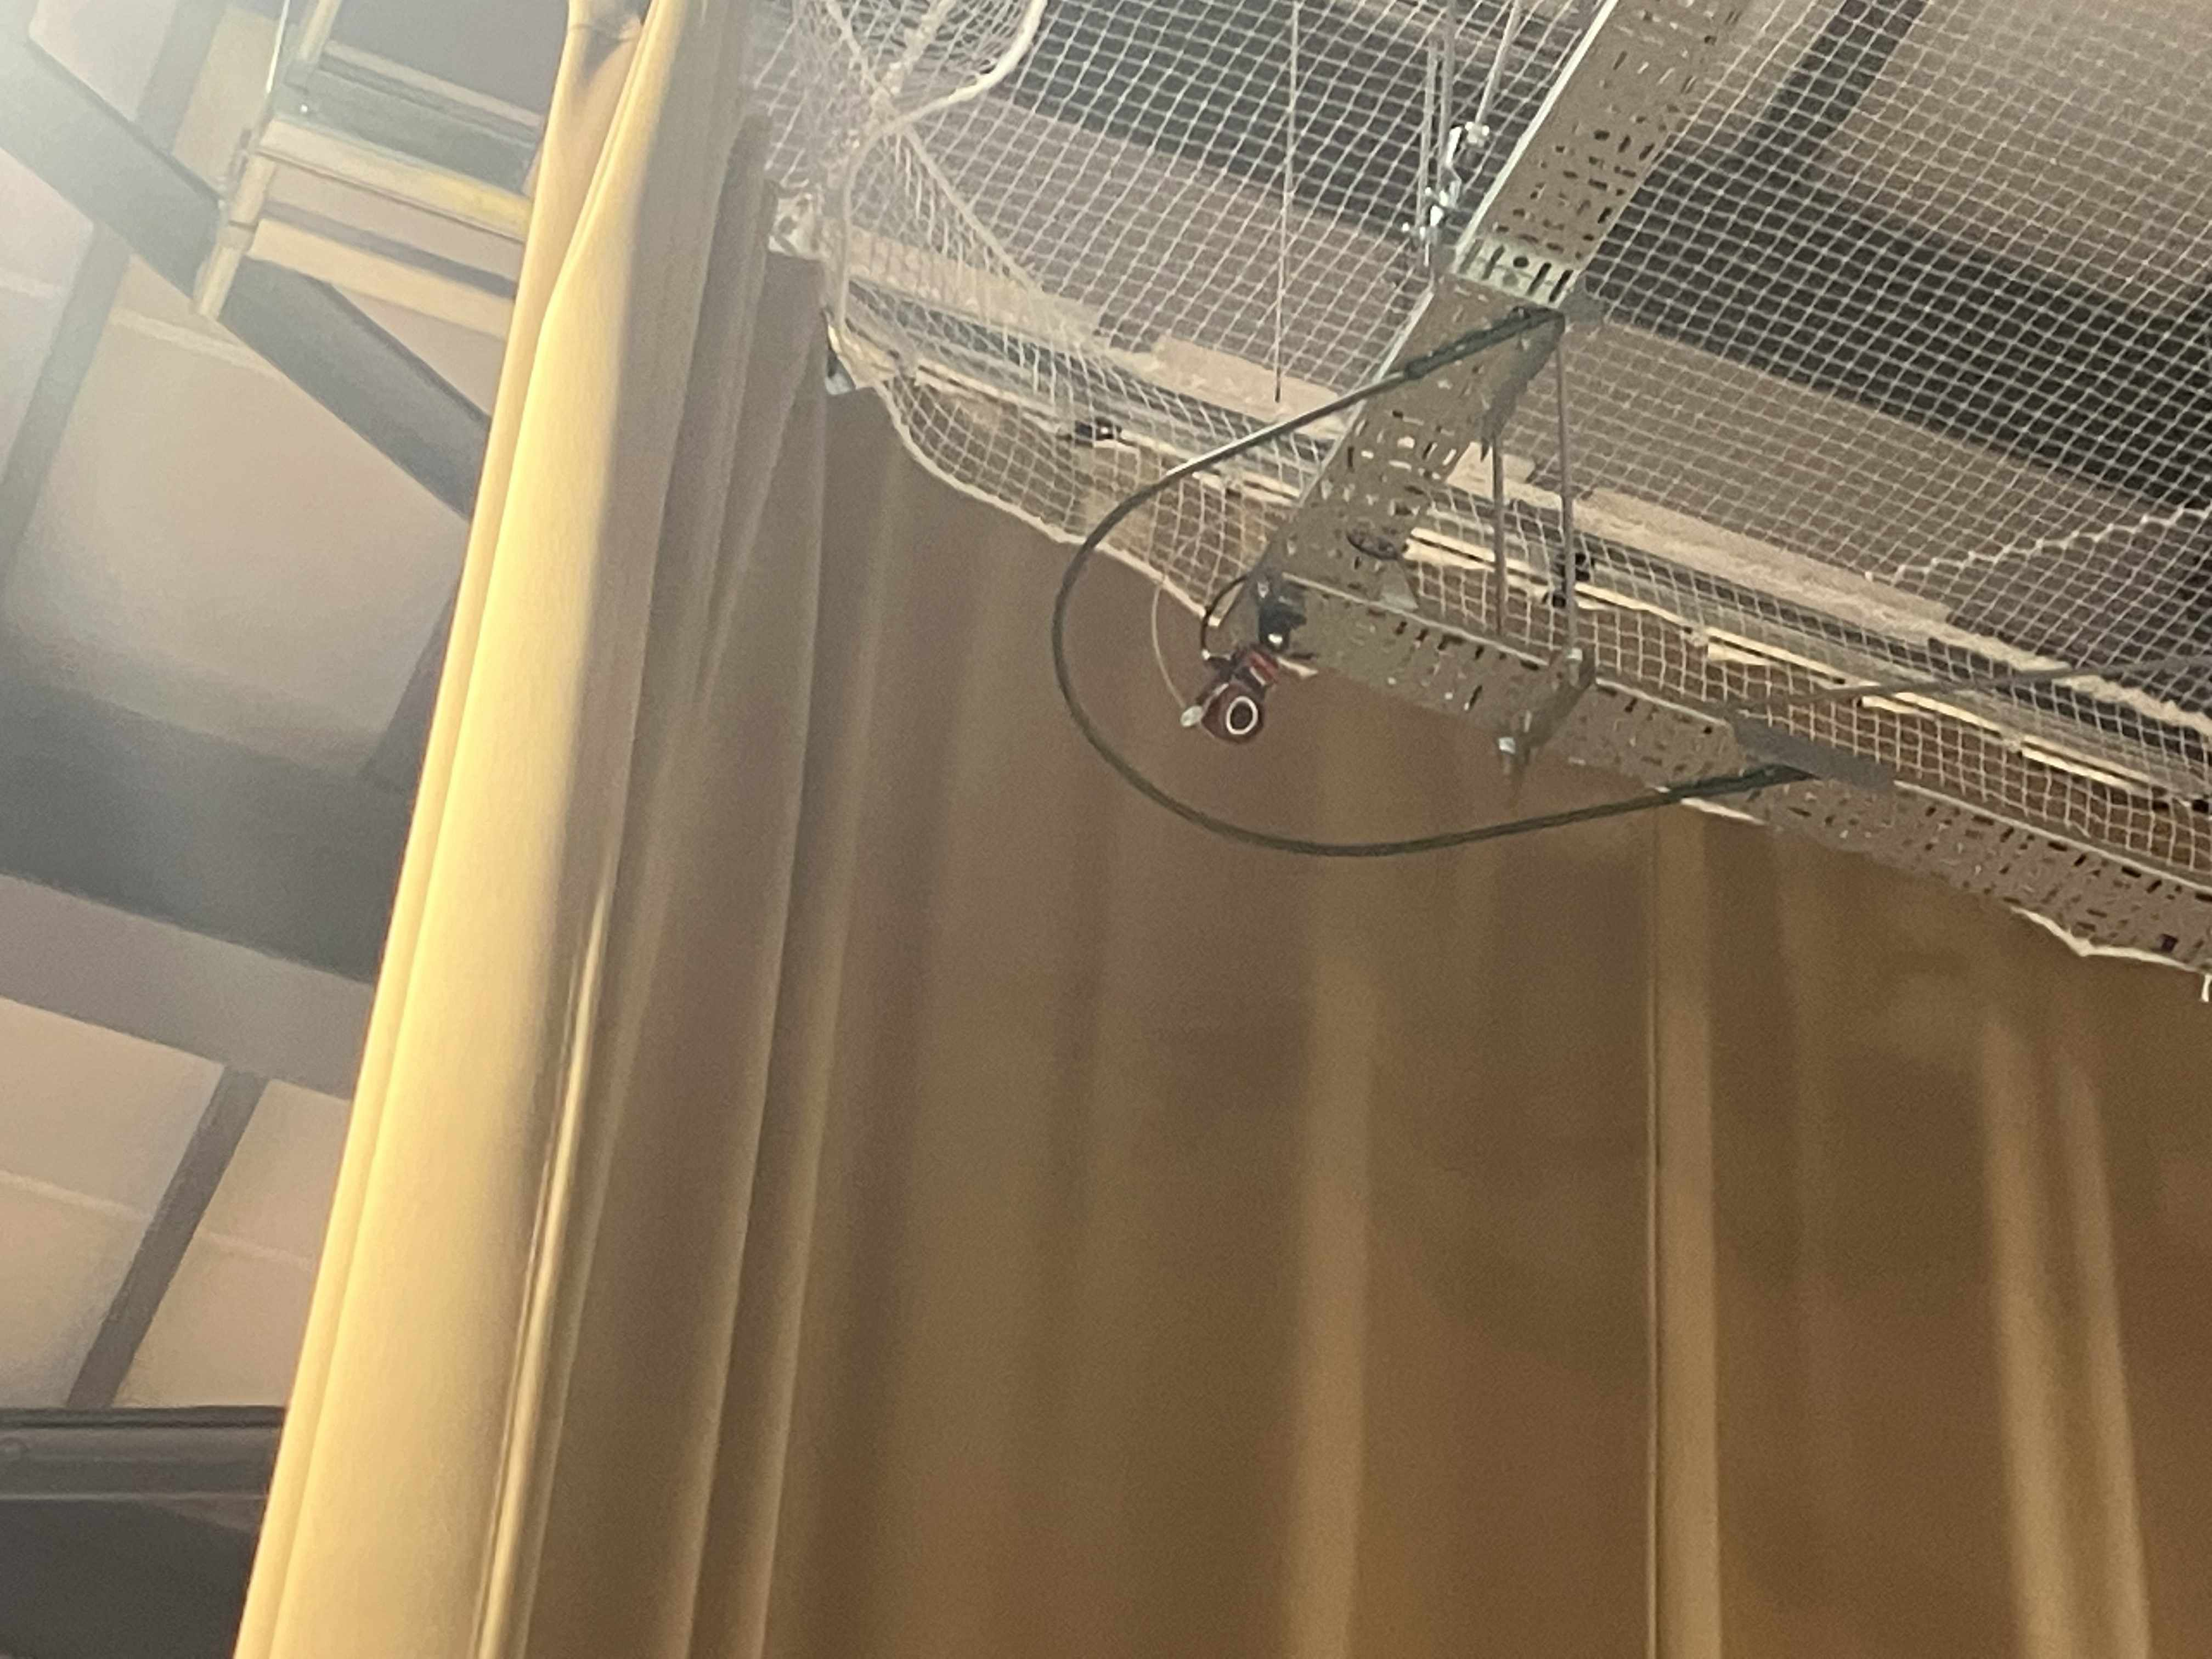
\includegraphics[width=100mm]{figure/IMG_3299.jpg}
% \caption{Motion capture camera}
% \label{cam}\vspace{0zh}\end{figure}

\begin{figure}[H]\centering
  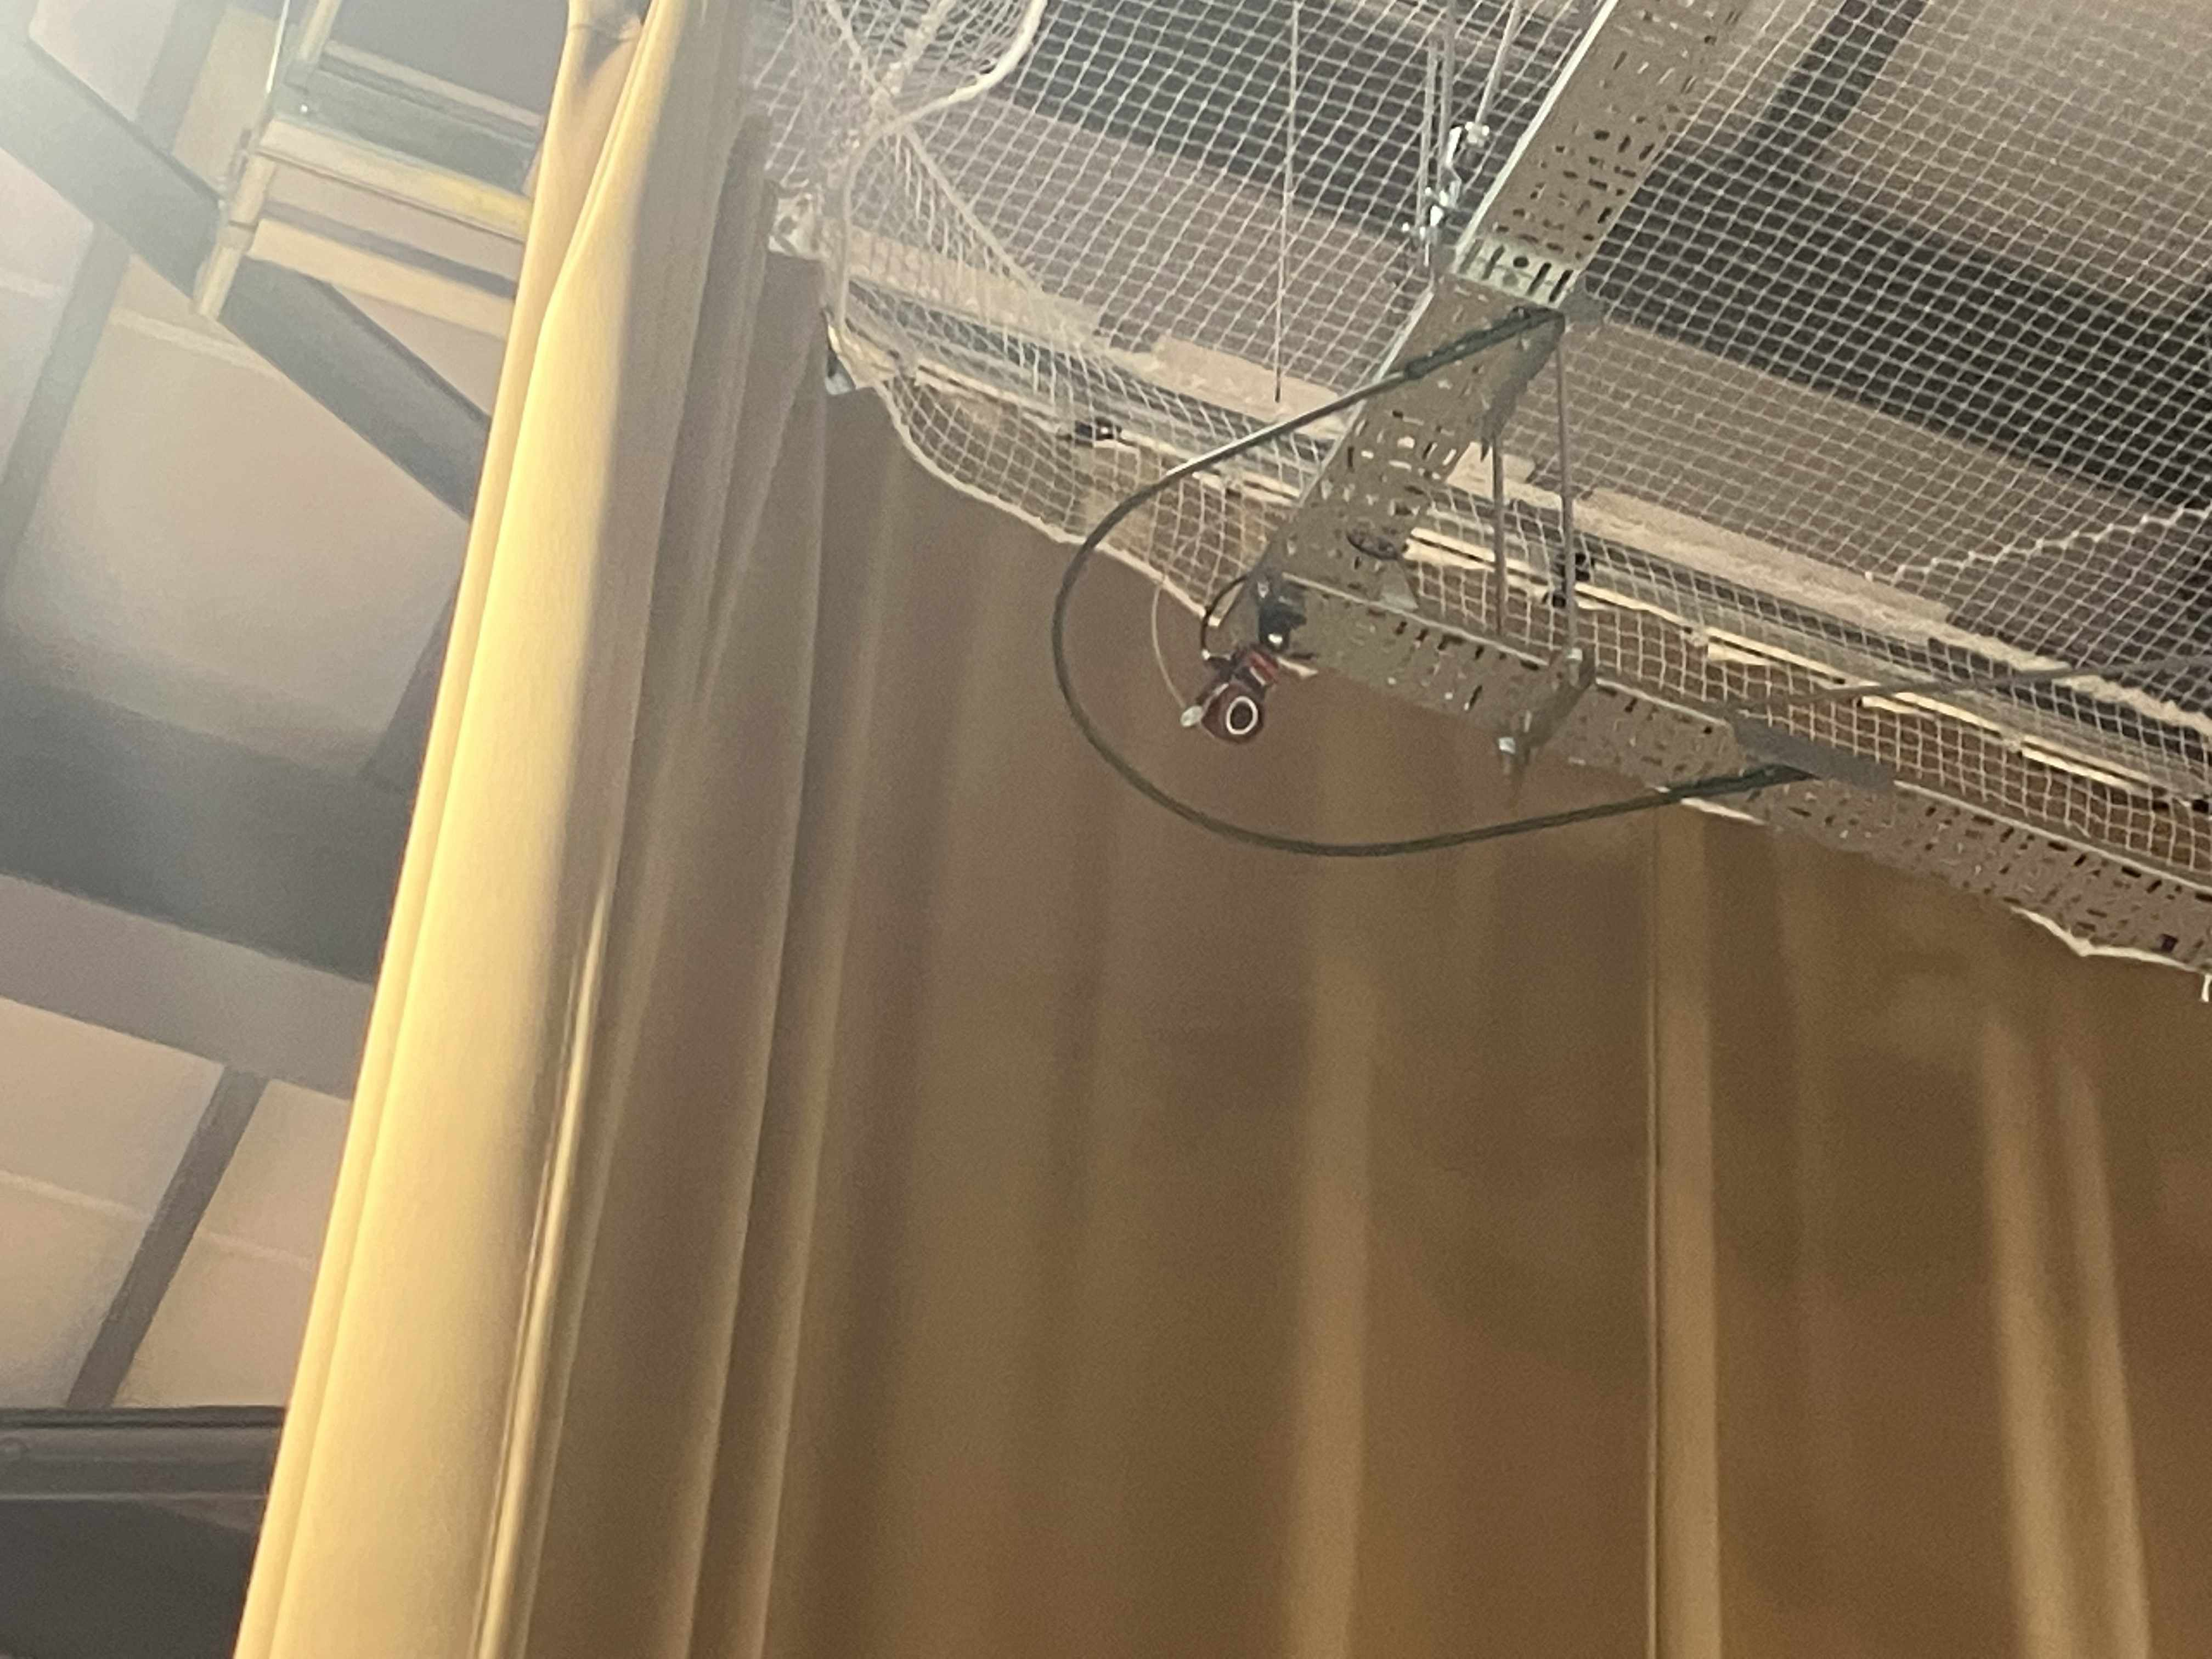
\includegraphics[width=100mm]{figure/IMG_3299.jpg}
  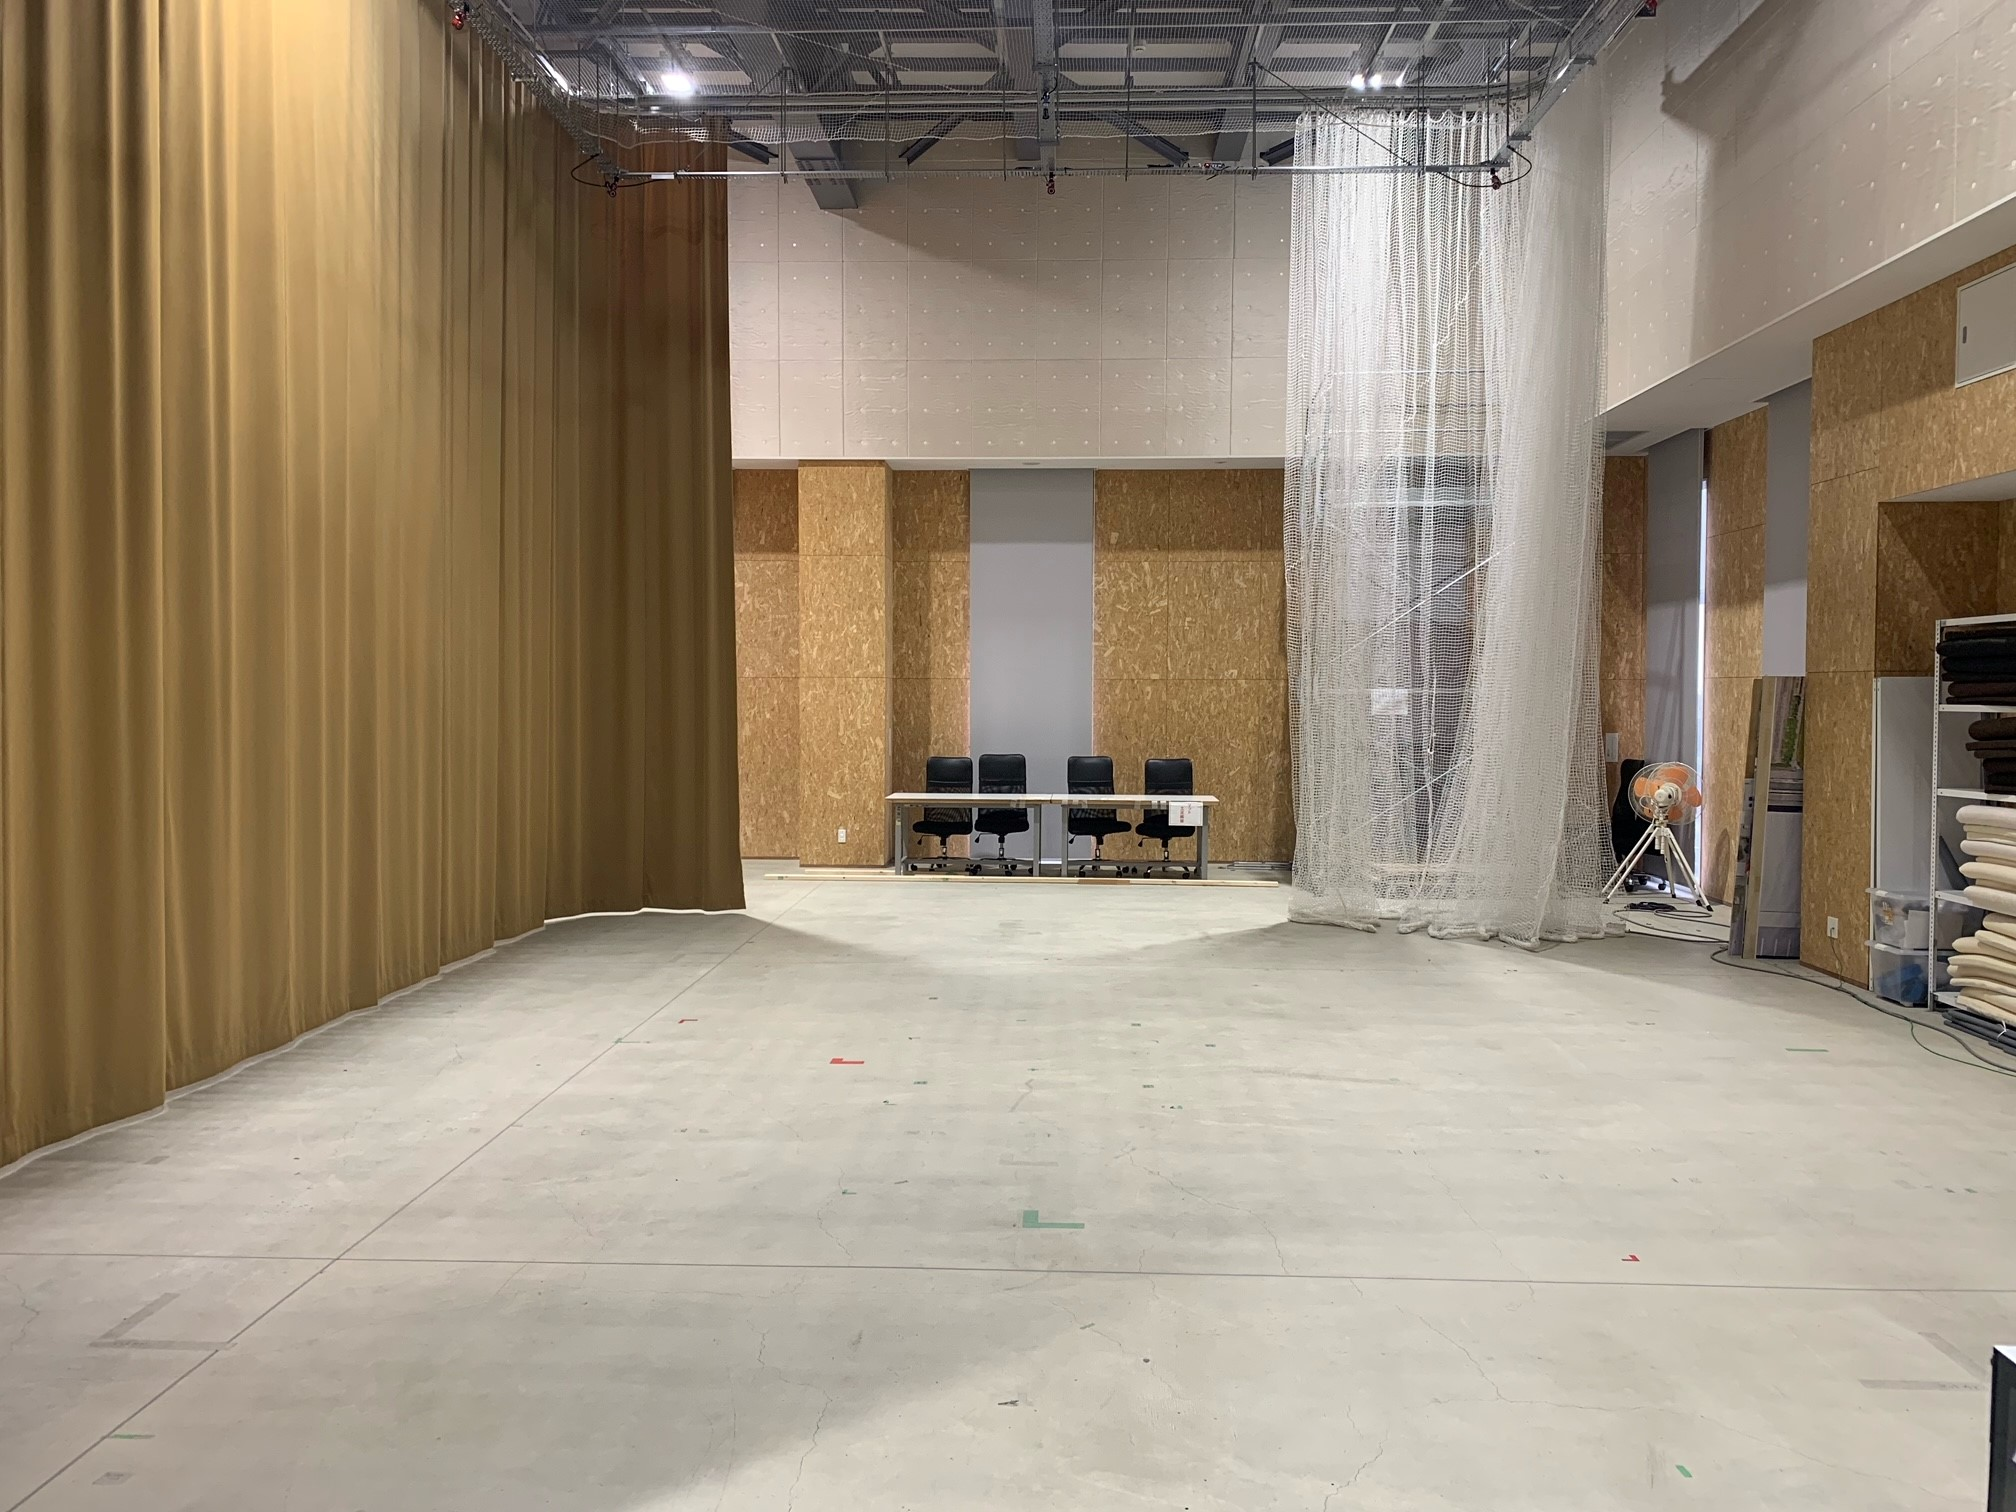
\includegraphics[width=100mm]{figure/Flight_space.jpg}
\caption{Motion capture camera}\label{cam}\end{figure}

\newpage

\section{直進動作におけるオドメトリ評価}\label{ex1}
\subsection{実験方法}
実験方法について説明する.まず,Roombaの上にモーションキャプチャー用のマーカーを6つ取り付ける.この操作は,今後の実験でも同様に行う.
マーカーを装着した後に,モーションキャプチャーにおける中心座標にRoombaを設置し直進させる.動作中は,オドメトリで算出された自己位置と姿勢を記録しながら,
モーションキャプチャーカメラでも移動中のRoombaの位置と姿勢を記録する.

\subsection{結果}
Fig.\ref{ex1_1}にRoombaの直進動作におけるオドメトリより算出した自己位置と自己位置の真値の推移を示す.ここで,Fig.\ref{ex1_1}は,x軸の正方向が進行方向である.
Fig.\ref{ex1_2}に直進動作におけるオドメトリより算出したRoombaの姿勢と真値のおける姿勢の遷移を示す.
Fig.\ref{ex1_3}に,X軸方向の誤差率を示し,
Fig.\ref{ex1_4}に,Y軸方向の誤差率を示す.
それぞれの誤差率は式\ref{x_error},\ref{y_error}より算出し,プロットしている.
Fig.\ref{ex1_6}とFig.\ref{ex1_7}に,それぞれ並進速度と角速度の遷移を示す.\\
Fig.\ref{ex1_1}より,進行した距離の誤差はほぼ無く,進行方向に対する左右のずれが約50mmあることが分かる.
この様子は,Fig.\ref{ex1_3},\ref{ex1_4}からも確認することができ,Fig.\ref{ex1_3}より
進行距離の誤差率は7\%であったのに対し,Fig.\ref{ex1_4}より左右のずれの誤差率は約210\%となっている.


\begin{align}\label{x_error}
  X\_Error Rate(t) = \cfrac{X\_True Val(t) - X\_Odometry(t)}{X\_True Val(t_{end})}* 100
\end{align}

\begin{align}\label{y_error}
  Y\_Error Rate(t) = \cfrac{Y\_True Val(t) - Y\_Odometry(t)}{Y\_True Val(t_{end})}* 100
\end{align}

\begin{figure}[H]\centering
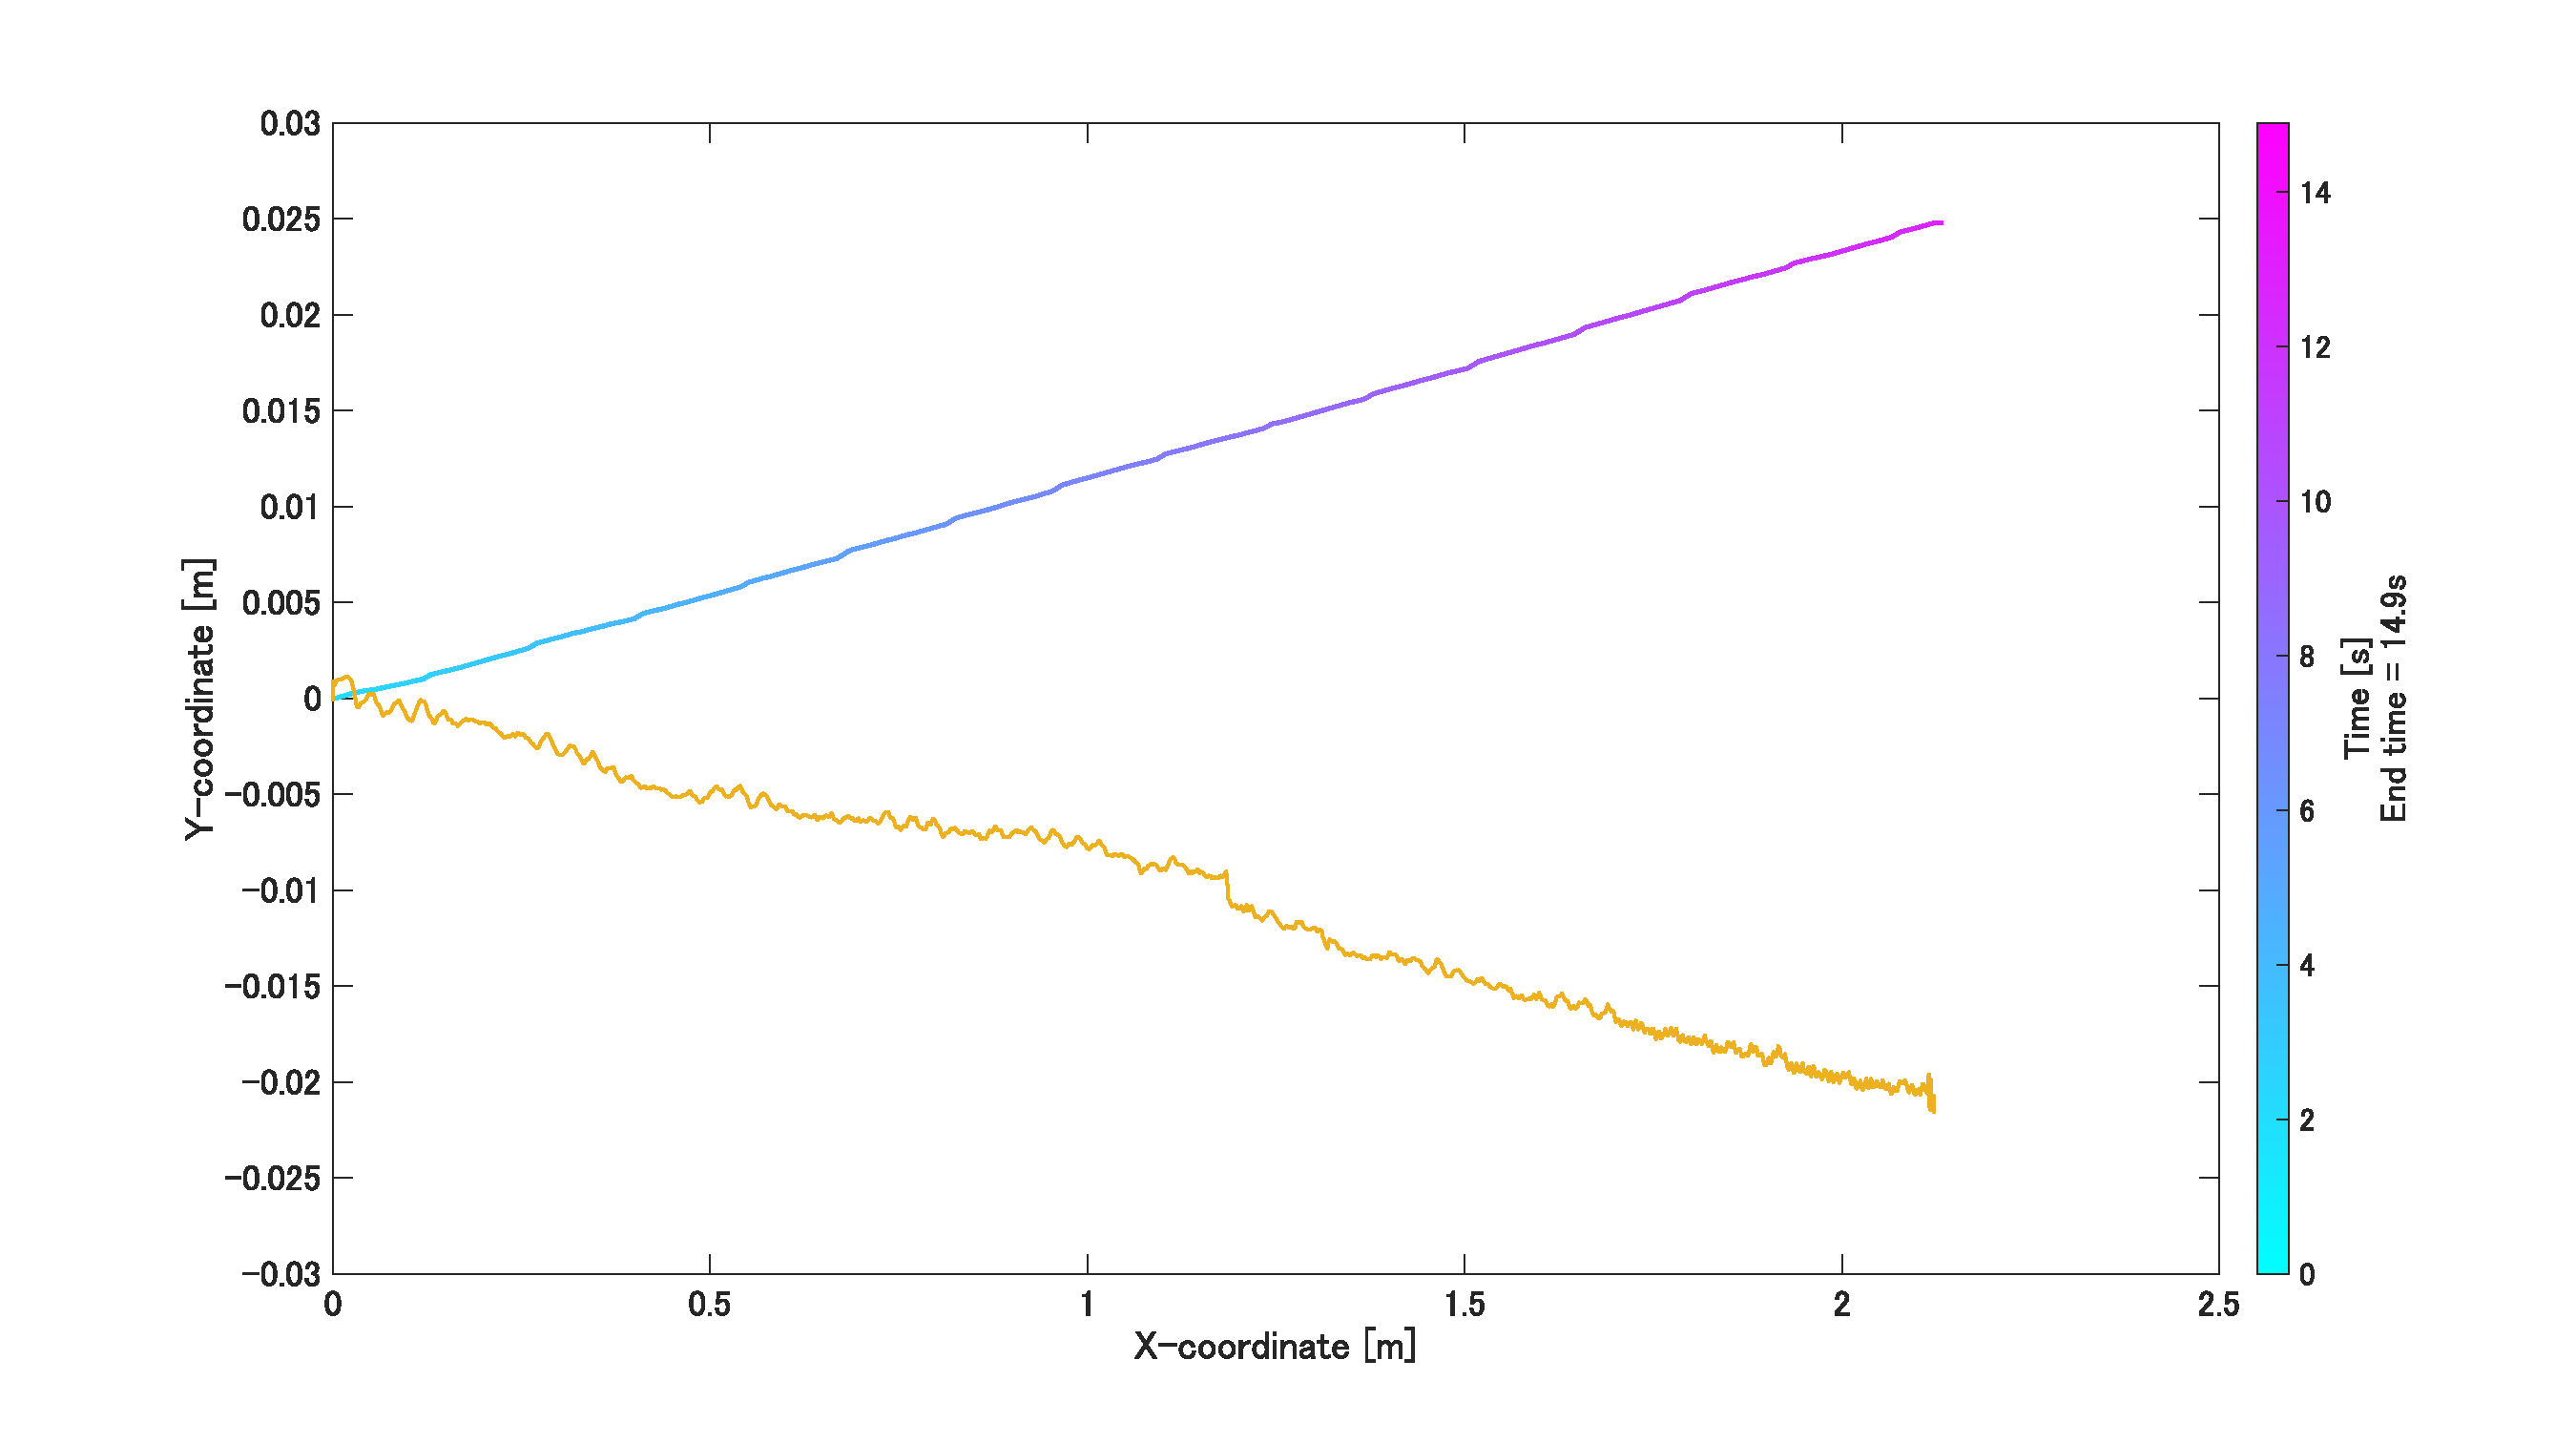
\includegraphics[width=100mm]{figure/1_1.eps}
\caption{translatory motion}
\label{ex1_1}\vspace{0zh}\end{figure}

\begin{figure}[H]\centering
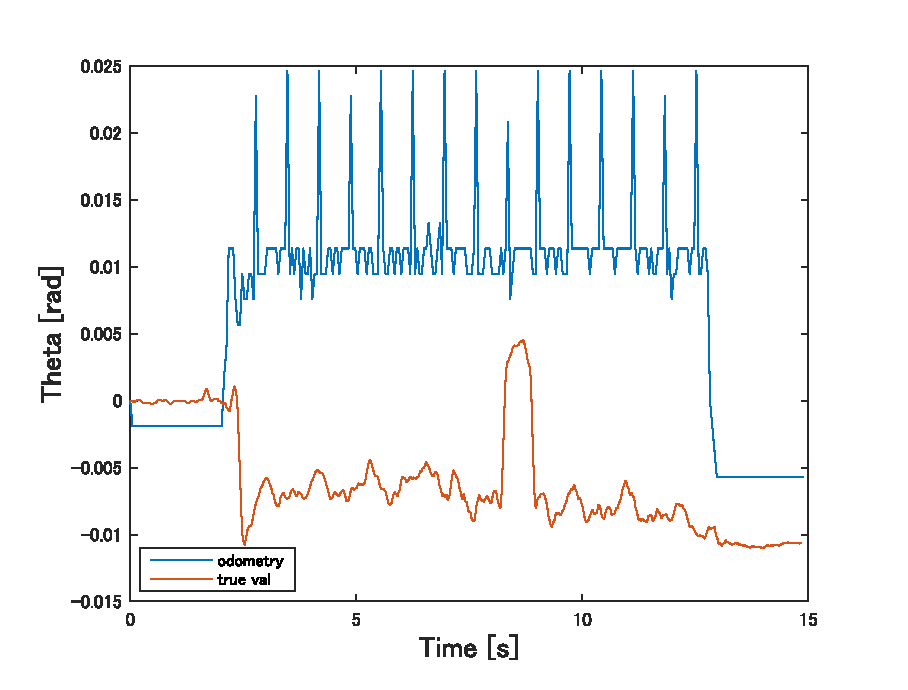
\includegraphics[width=100mm]{figure/1_2.eps}
\caption{Angle transition in translatory motion}
\label{ex1_2}\vspace{0zh}\end{figure}

\begin{figure}[H]\centering
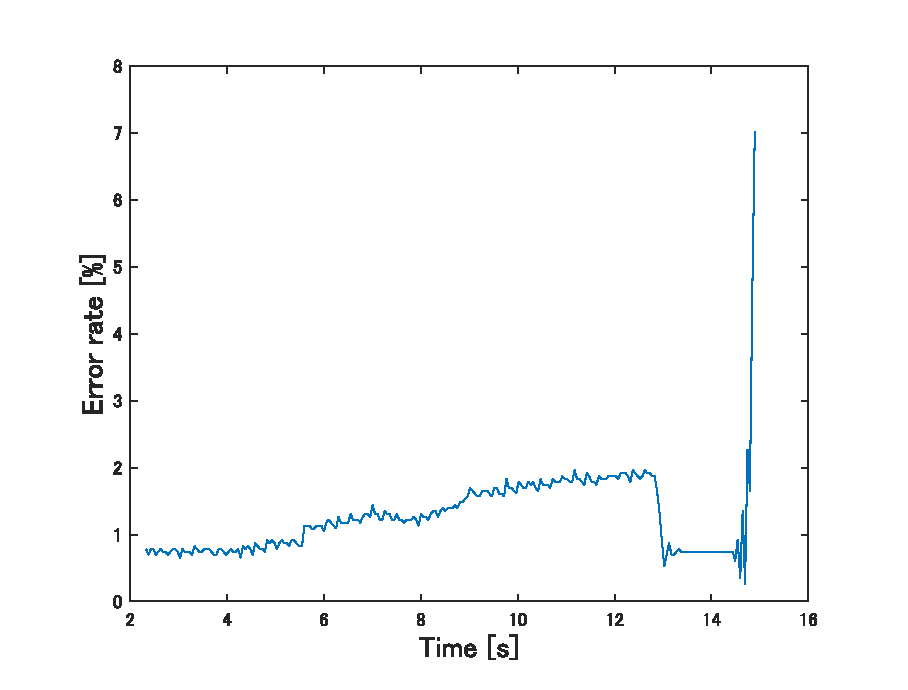
\includegraphics[width=100mm]{figure/1_3_xe.eps}
\caption{Error rate in x-axis direction}
\label{ex1_3}\vspace{0zh}\end{figure}

\begin{figure}[H]\centering
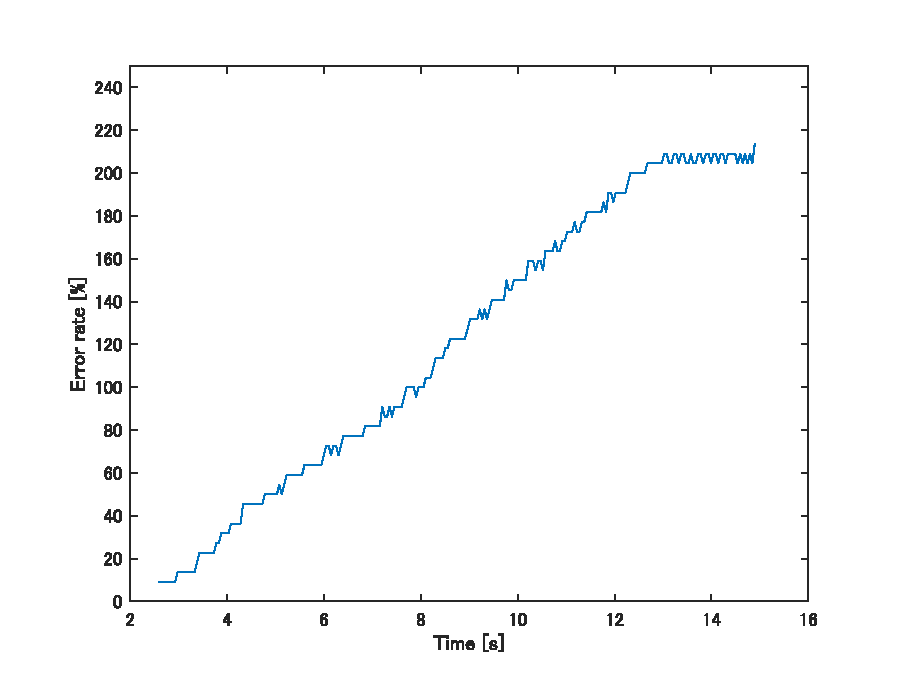
\includegraphics[width=100mm]{figure/1_4_ye.eps}
\caption{Error rate in y-axis direction}
\label{ex1_4}\vspace{0zh}\end{figure}


\begin{figure}[H]\centering
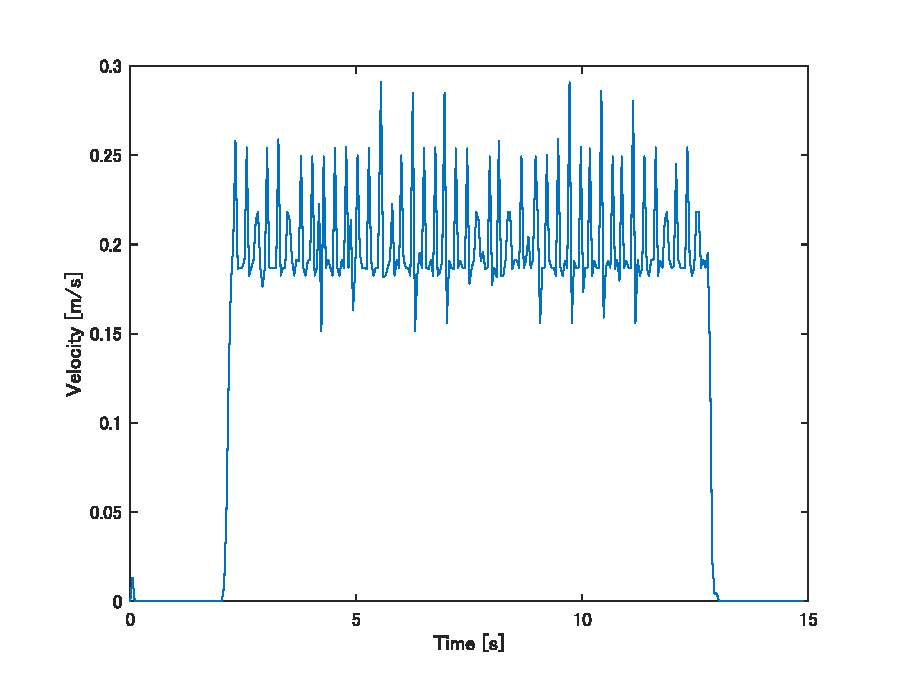
\includegraphics[width=100mm]{figure/1_6.eps}
\caption{Velocity in translatory motion}
\label{ex1_6}\vspace{0zh}\end{figure}

\begin{figure}[H]\centering
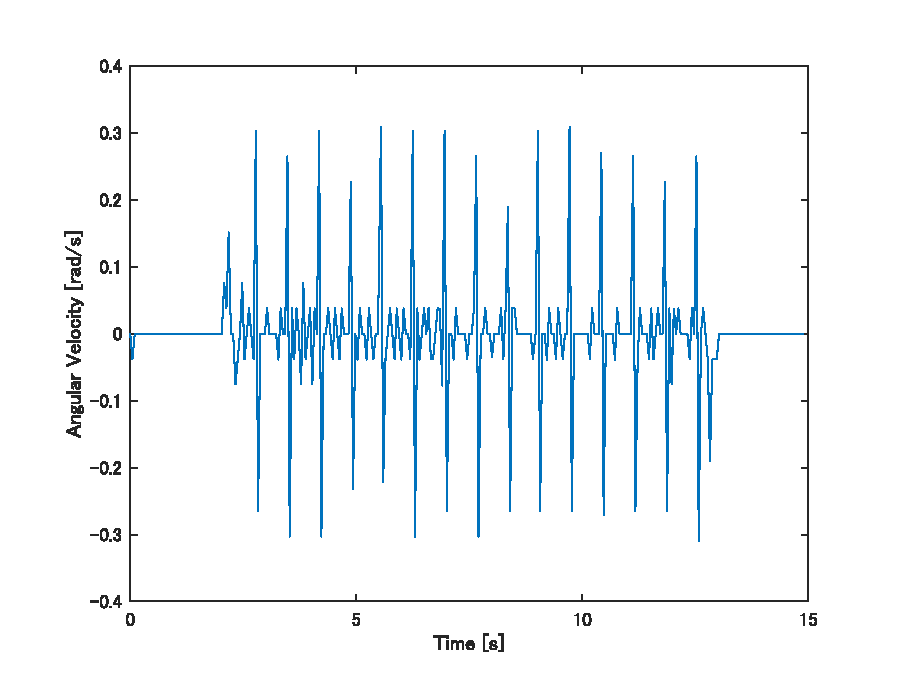
\includegraphics[width=100mm]{figure/1_7.eps}
\caption{Angular velocity in translatory motion}
\label{ex1_7}\vspace{0zh}\end{figure}

\newpage

\subsection{考察}
直進動作において,左右のずれが大きくなったことについて考察する.
まず,Fig.\ref{ex1_1}よりオドメトリで算出した自己位置と自己位置の真値で,進行方向の向きが大きく異なっていることが分かる.
ここで,Fig.\ref{ex1_2}より2.5秒付近で,大きく姿勢が変化していることが分かる.
Fig.\ref{ex1_6}より,2.5秒付近はroombaが動作を始めたタイミングであることから,始動トルクによって
両車輪が滑ってしまい,かつ右車輪の回転角が左車輪の回転角よりも大きかったために,前進しないまま本体の姿勢が左向きに向いたのだと考えられる.
この様子は,Fig.\ref{ex1_3},Fig.\ref{ex1_7}からも確認することができ確認できる.
併せて,真値では右向きに進んでいるのは,Roombaの設置時にモーションキャプチャー上の座標系に対し,Roombaが右向きを向いた状態で設置された
ためだと考えられる.このために,Fig.\ref{ex1_1}で示したオドメトリより算出した自己位置と自己位置の真値の遷移による軌跡
が描かれ,誤差率が非常に大きくなったのだと考えられる.\\
また,設置時に左右方向へ一切向かず,始動トルクによって滑らなかった場合の誤差について考える.
Fig.\ref{ex1_8}に,設置時のずれと始動トルクの影響がなかった場合のY軸の遷移のグラフを示す.
ここで,線形に変化している部分が,Roombaが動作している範囲であり,この変化を近似すると,式\ref{approximate_y_error}
となり,1秒あたり3.31mmずつ誤差が生じることになる.

\begin{align}\label{approximate_y_error}
y(t) = 2.38(t) + 0.93
\end{align}

\begin{figure}[H]\centering
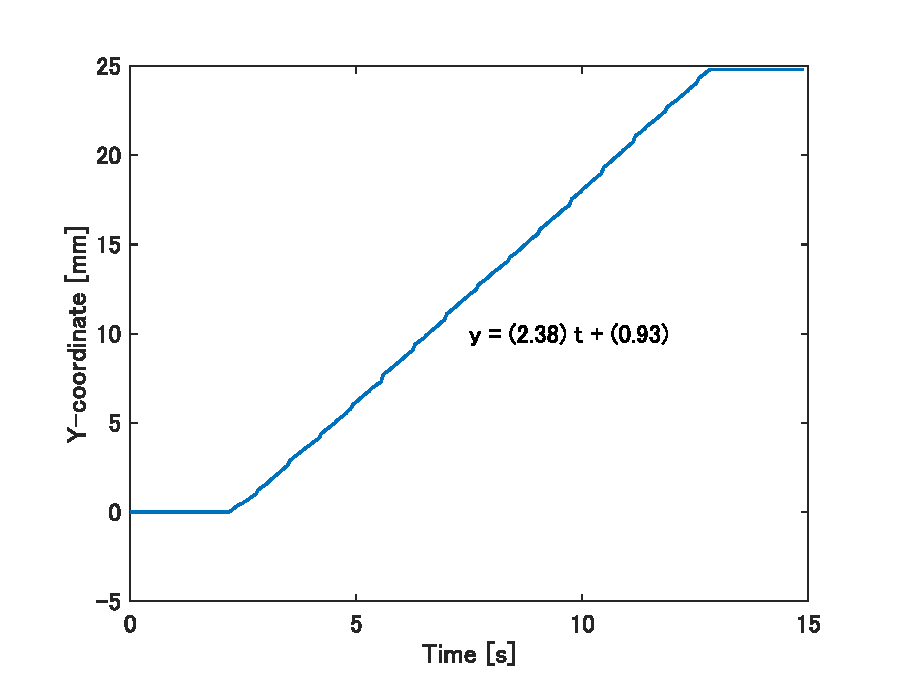
\includegraphics[width=100mm]{figure/1_8.eps}
\caption{Y-axis error excluding installation and starting torque effects}
\label{ex1_8}\vspace{0zh}\end{figure}

\newpage

\section{超信地旋回におけるオドメトリ評価実験}\label{ex2}
\subsection{実験方法}
マーカーを装着した後に,モーションキャプチャーにおける中心座標に
Roombaを設置し超信地旋回させる.動作中は,オドメトリで算出された自己位置と
姿勢を記録しながら,モーションキャプチャーカメラでも移動中のRoombaの位置と
姿勢を記録する.

\subsection{結果}
Fig.\ref{ex2_1}にRoombaが超信地旋回した際のオドメトリより算出した自己位置と自己位置の真値の推移を示す.
Fig.\ref{ex2_2}に超信地旋回におけるオドメトリより算出したRoombaの姿勢と真値のおける姿勢の遷移を示す.
Fig.\ref{ex2_5_1}に,動作してから0秒から6秒までの姿勢の誤差率を示し,
Fig.\ref{ex2_5_2}に,6秒から動作終了までの姿勢の誤差率を示す.誤差率は式\ref{theta_error}より算出し,プロットしている.

超信地旋回においては.Fig.\ref{ex2_1}より自己位置の誤差は30mm以内であった.動作停止時における誤差は,X軸方向に10.4mm,Y軸方向に3.5mmとなった.
また,Fig.\ref{ex2_2}より真値とオドメトリにおける姿勢の誤差はほぼ無かった.これは,Fig.\ref{ex2_5_1}で誤差率が6\%以内であったこと,
Fig.\ref{ex2_5_2}で誤差率が最終的に0\%に収束していることからも分かる.

\begin{align}\label{theta_error}
  Theta\_Error Rate(t) = \cfrac{Theta\_True Val(t) - Theta\_Odometry(t)}{Theta\_True Val(t_{end})}* 100
\end{align}

\begin{figure}[H]\centering
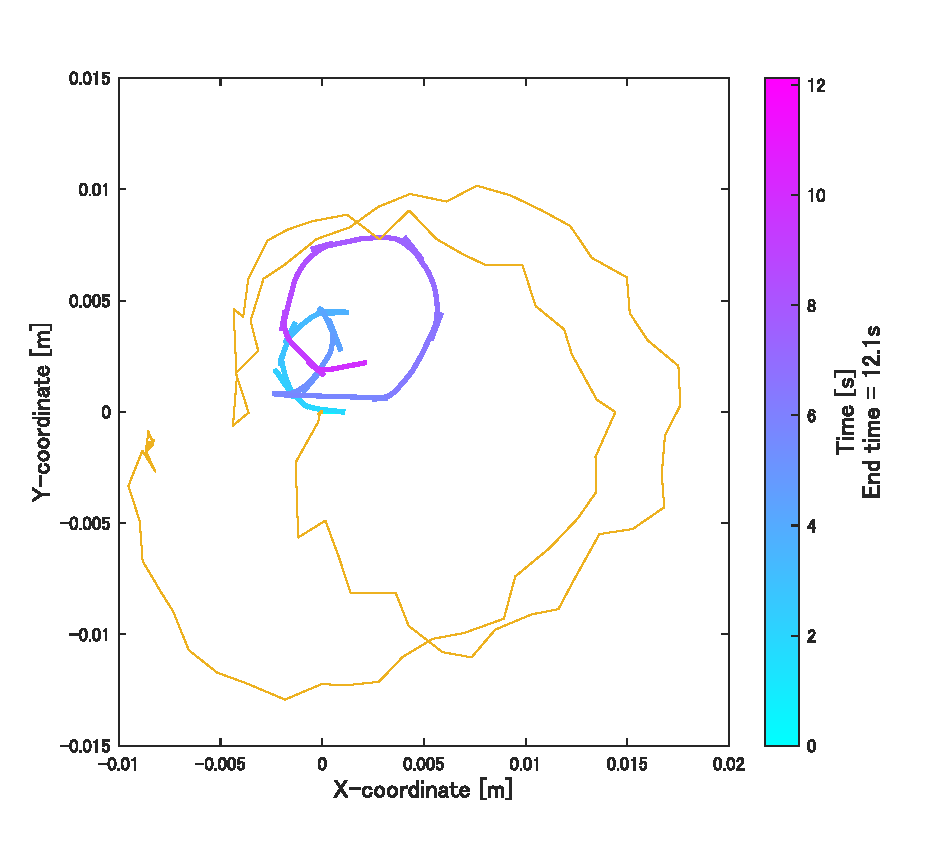
\includegraphics[width=100mm]{figure/2_1.eps}
\caption{Angle Transition in Turning on the spot}
\label{ex2_1}\vspace{0zh}\end{figure}

\begin{figure}[H]\centering
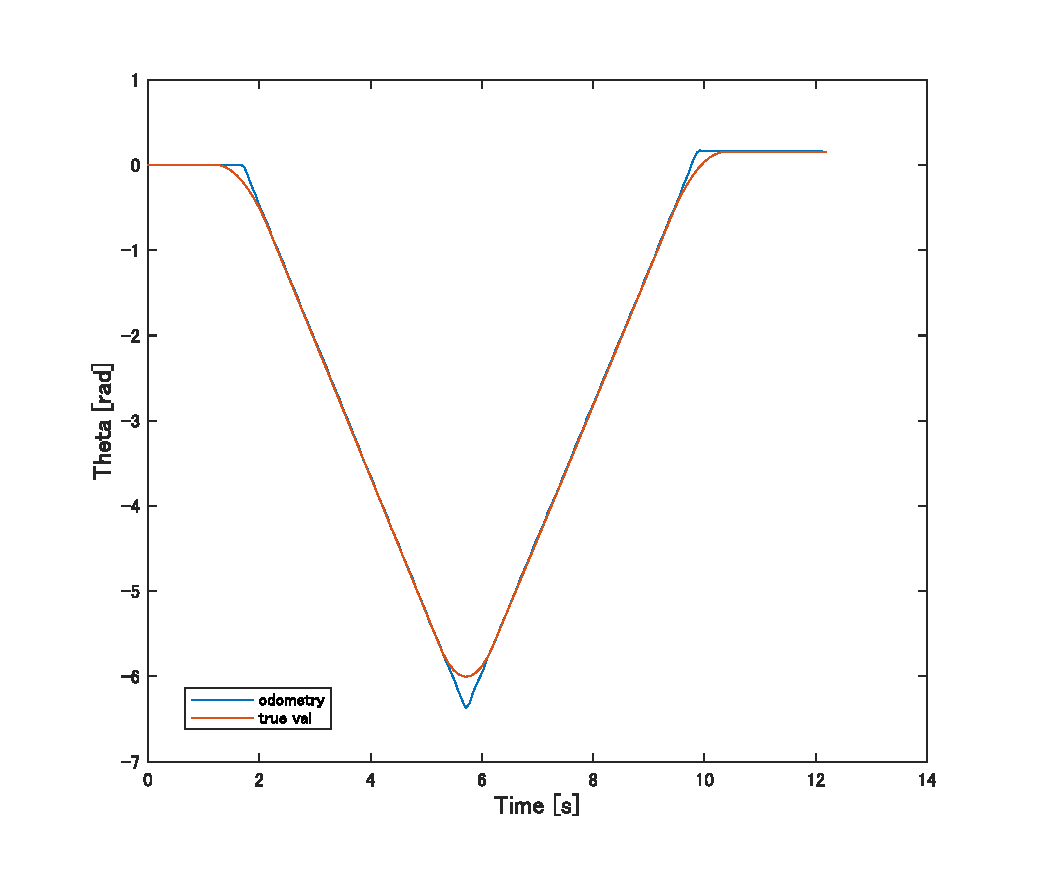
\includegraphics[width=100mm]{figure/2_2.eps}
\caption{Angle Transition in turning movements}
\label{ex2_2}\vspace{0zh}\end{figure}


\begin{figure}[H]\centering
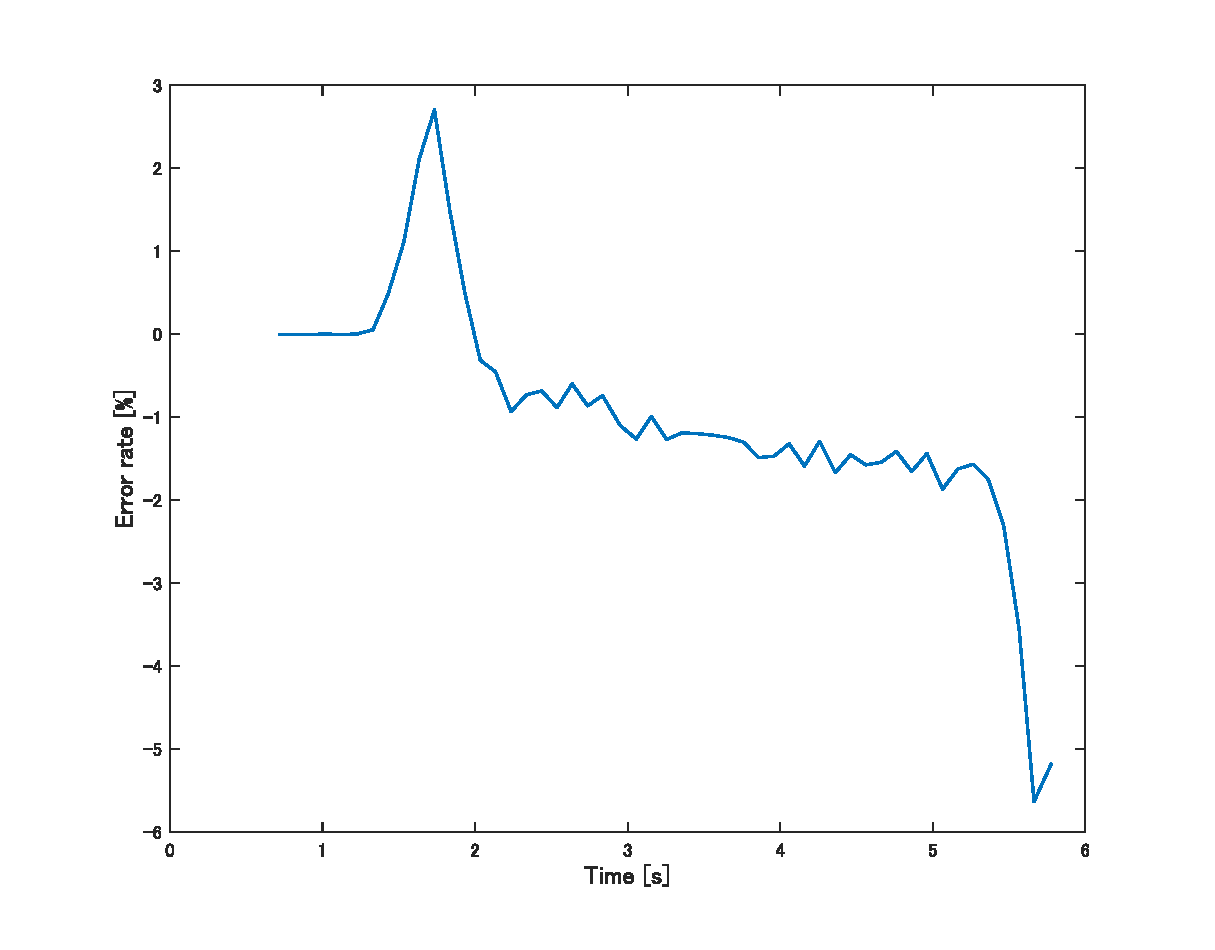
\includegraphics[width=100mm]{figure/2_5_1_te.eps}
\caption{Error rate of θ from 0 to 6 sec}
\label{ex2_5_1}\vspace{0zh}\end{figure}

\begin{figure}[H]\centering
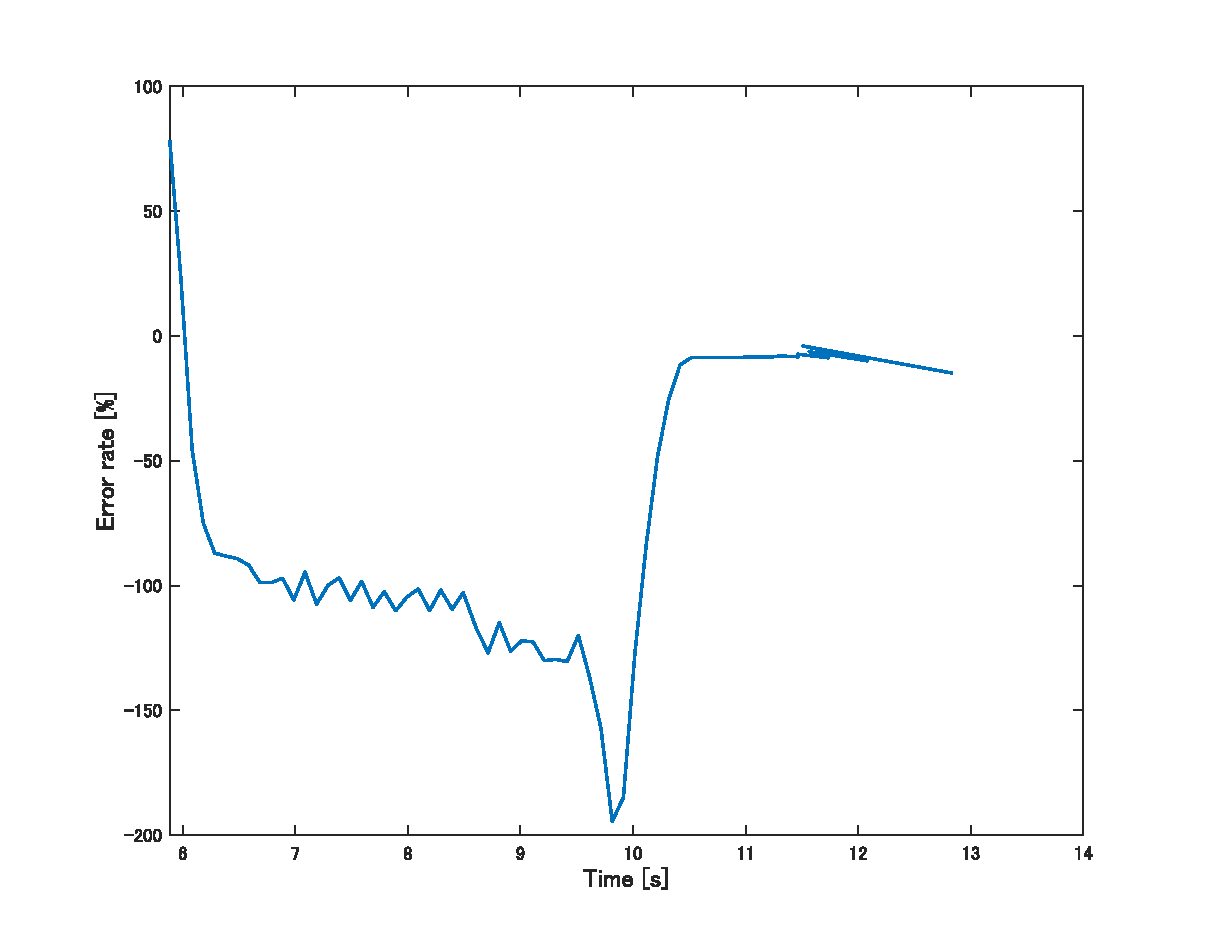
\includegraphics[width=100mm]{figure/2_5_2_te.eps}
\caption{Error of θ from 6 to 14 sec}
\label{ex2_5_2}\vspace{0zh}\end{figure}

\newpage

\subsection{考察}
旋回動作における自己位置と姿勢の誤差が小さかったことについて考察する.
並進移動する際は,Fig.\ref{T_f1}に示すように,駆動力は摩擦力の反力として,回転軸に対して垂直に生じる.
しかし,Fig.\ref{T_f2}に示すように,超信地旋回などの旋回動作をする際は左右の車輪の速度差によって回転中心が決まり,回転中心に近づける微小な力$F_2$が生じるため,
$F_2$の大きさだけ駆動力が小さくなり,旋回半径の接線方向に$F_2$と駆動力の合力である$F_1$が生じる.ここで,$F_1$と並進時の駆動力の大きさは等しいと考えられる.
よって今回の実験では,旋回動作によって駆動力が低下したために,車輪が滑りづらくなり自己位置と姿勢の誤差が小さくなったのだと考えられる.

\begin{figure}[H]\centering
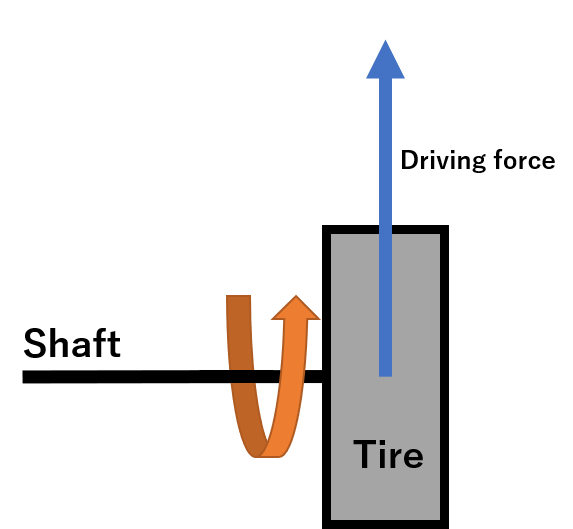
\includegraphics[width=100mm]{figure/Tire_force1.png}
\caption{Force applied to wheels during translation}
\label{T_f1}\vspace{0zh}\end{figure}

\begin{figure}[H]\centering
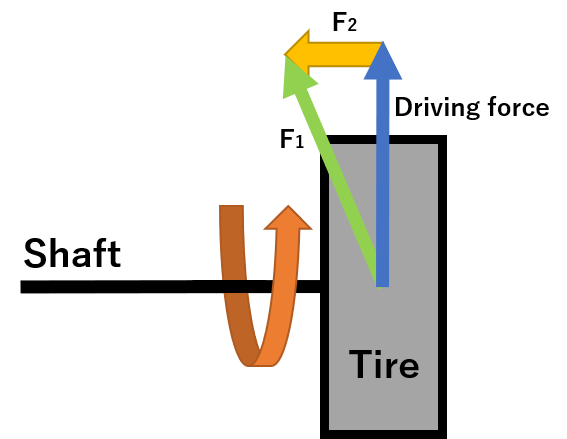
\includegraphics[width=100mm]{figure/Tire_force2.png}
\caption{Force applied to wheels during turning}
\label{T_f2}\vspace{0zh}\end{figure}


\newpage

\section{緩旋回におけるオドメトリ評価実験}\label{ex3}
\subsection{実験方法}
マーカーを装着した後に,モーションキャプチャーにおける中心座標に
Roombaを設置し,緩旋回させながら初期地点に戻るように動作させる.
動作中は,オドメトリで算出された自己位置と
姿勢を記録しながら,モーションキャプチャーカメラでも移動中のRoombaの位置と
姿勢を記録する.

\subsection{結果}
Fig.\ref{ex3_1}にRoombaが緩旋回した際のオドメトリより算出した自己位置と座標の自己位置の推移を示す.
Fig.\ref{ex3_2}に緩旋回動作におけるオドメトリにより算出したRoombaの姿勢と真値における姿勢の遷移を示す.
Fig.\ref{ex3_1}より,動作停止時における誤差は,X軸方向に1.7mm,Y軸方向に3.7mmとなった.



\begin{figure}[H]\centering
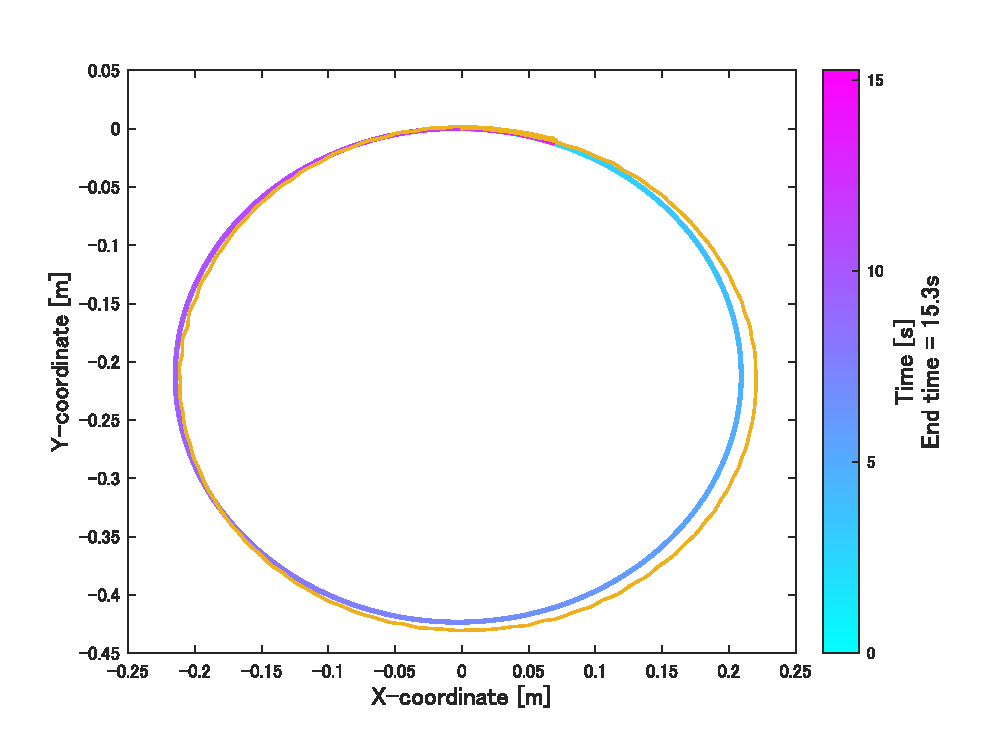
\includegraphics[width=100mm]{figure/3_1.eps}
\caption{Gentle turn movements}
\label{ex3_1}\vspace{0zh}\end{figure}

\begin{figure}[H]\centering
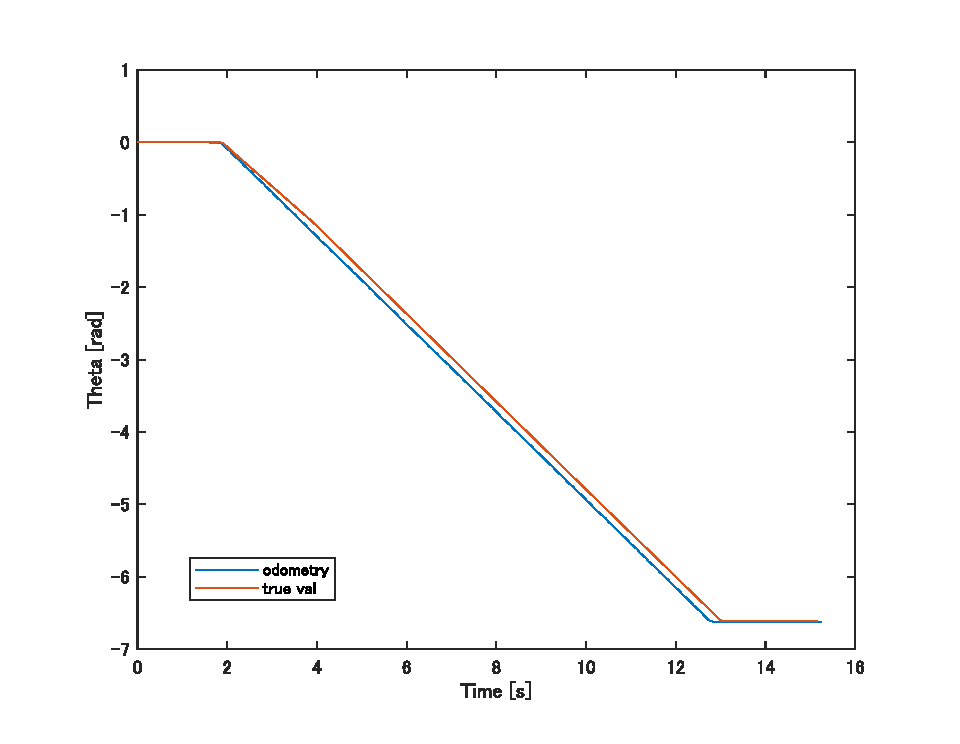
\includegraphics[width=100mm]{figure/3_2.eps}
\caption{Angle Transition in Gentle turn movements}
\label{ex3_2}\vspace{0zh}\end{figure}


\subsection{考察}
今回の実験では,第\ref{ex2}章の説明した超信地旋回よりも座標の誤差は小さく,X軸Y軸方向ともに5mm以下となった.
これは,第\ref{ex2}章の考察で述べたように,旋回することによって,並進時に比べ駆動力が低下したためだと考えられる.


\newpage

\section{四角形経路走行におけるオドメトリ評価実験}\label{ex4}
\subsection{実験方法}
マーカーを装着した後に,モーションキャプチャーにおける中心座標に
Roombaを設置し,四角形経路走行させて初期地点に戻るように動作させる.
動作中は,オドメトリで算出された自己位置と
姿勢を記録しながら,モーションキャプチャーカメラでも移動中のRoombaの位置と
姿勢を記録する.

\subsection{結果}
Fig.\ref{ex4_1}に四角形経路走行におけるオドメトリより算出した自己位置と自己位置の真値の推移を示す.
Fig.\ref{ex4_2}に四角形経路走行におけるオドメトリにより算出したRoombaの姿勢と真値のおける姿勢の遷移を示す.
Fig.\ref{ex4_1}より,四角形経路走行における動作停止時における誤差は,x軸で27.4mm,y軸で42.2mmであった.


\begin{figure}[H]\centering
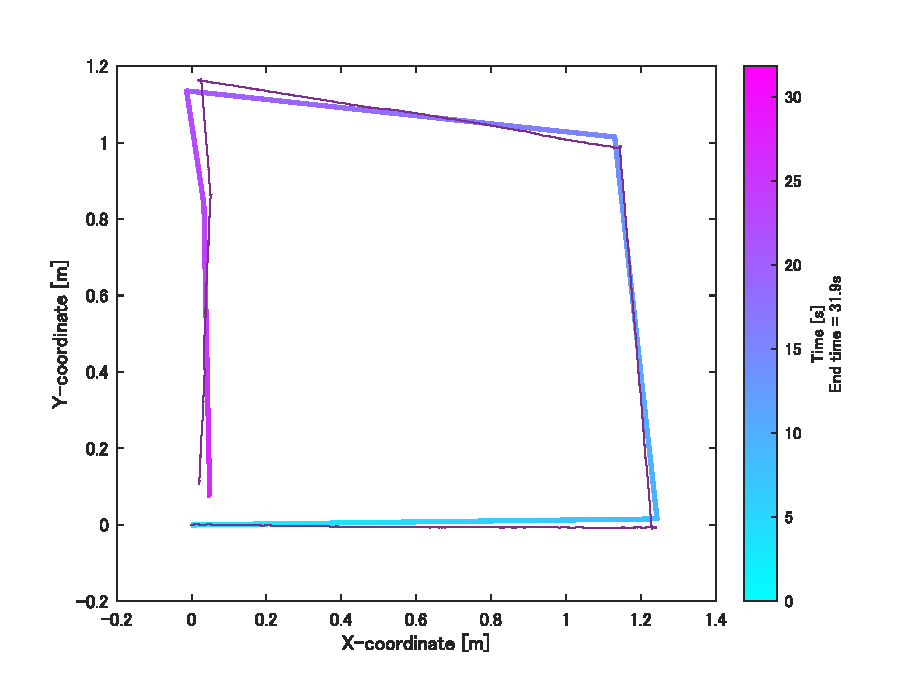
\includegraphics[width=100mm]{figure/4_1.eps}
\caption{Movements of rectangular route running}
\label{ex4_1}\vspace{0zh}\end{figure}

\begin{figure}[H]\centering
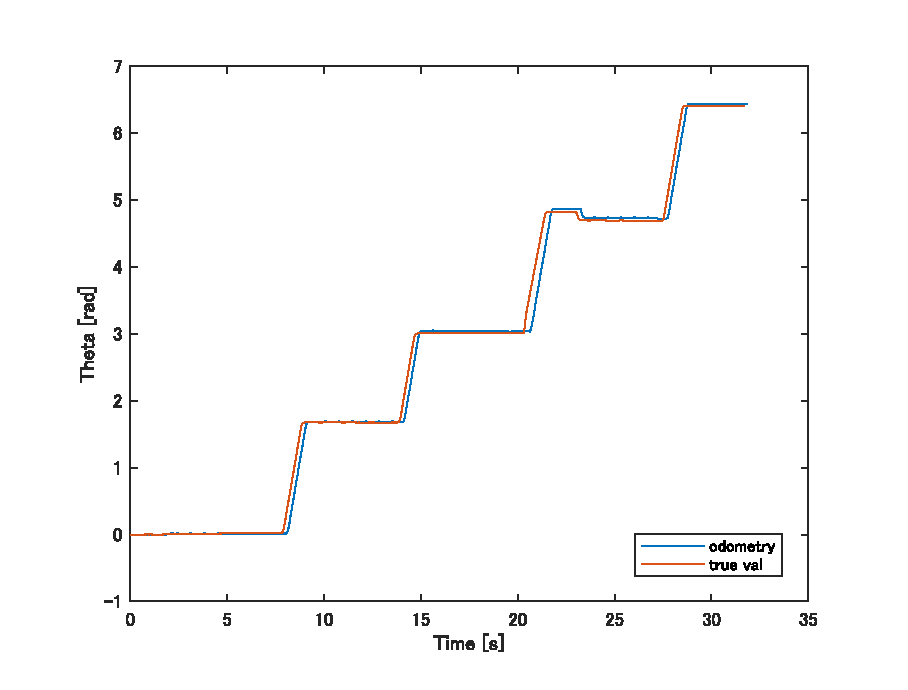
\includegraphics[width=100mm]{figure/4_2.eps}
\caption{Angle Transition in rectangular route running}
\label{ex4_2}\vspace{0zh}\end{figure}

\subsection{考察}
今回の実験では,これまでの実験で最も誤差が大きくなった.これについて考察する.\\
四角形経路を走行するにあたり,旋回→停止→直進を繰り返し経路走行を行った.そのために,
第\Ref{ex1}章の直進動作実験で考察したように,停止して直進する際に始動トルクによって車輪が滑り,誤差が生まれ,
それが蓄積し大きな誤差が生まれたのだと考えられる.

\newpage

\section{おわりに}
今回,一連の実験を通して,以下のことが分かった.
\begin{enumerate}
\item 並進させる際は,現在の速度制御の設定である200mm/sだと,始動トルクによって車輪が滑るため,誤差が生じる.
\item 始動トルクや設置時の誤差の影響がない場合でも,Y軸の正方向に3.31mmずつ誤差が生じる.
\item 旋回動作においては.駆動力が低下するため車輪が滑りにくくなり,誤差が生じにくい.
\end{enumerate}





\end{document}